\chapter{Introdução}\label{chp:intro}

Com a recente diminuição do custo das plataformas de processamento e sensoriamento embarcado \citep{perlmutter2012high} um novo ramo de mercado surgiu ao redor do desenvolvimento de VANTs \citep{brief2011growth}.

Ainda que os avanços na tecnologia de baterias tenha permitido que este mercado surgisse, sua baixa densidade de potencia \citep{nitta2015li} \citep{tarascon2011issues} exige que os projetos de VANTs sejam altamente otimizados em relação ao consumo energético.

Um problema frequente em projetos aeronáuticos, porém, é a incerteza quanto aos dados aerodinâmicos dos diversos componentes que compõem a aeronave. A resolução deste problema é abordada em geral de três maneiras: estimativas teóricas, simulação fluidodinâmica e experimentação, possuindo cada um destes suas vantagens e desvantagens \citep{anderson1995computational} .

As estimativas teóricas em geral se encontram no projeto como método inicial de avaliação. A vantagem desta se dá pela vasta literatura disponível e por consistir na aplicação de fórmulas (em geral) simples. A desvantagem está na incerteza sobre a exatidão do resultado, isto é, não se sabe o quanto o mesmo esta próximo da realidade, ou mesmo se o valor é subestimado ou superestimado.

A simulação é uma alternativa muito utilizada, e sua vantagem se dá na maior exatidão dos resultados quando o modelo e os parâmetros de simulação já são bem conhecidos e comportados para a geometria estudada. O problema principal deste método se encontra na maior dificuldade de emprego, pois se limita a modelos que já tenham sido validados contra resultados experimentais. Para geometrias pouco estudadas, com parâmetros de simulação desconhecidos, corre-se o risco inclusive de se obter resultados ordens de grandeza afastados da realidade \citep{anderson1995computational}.

Por ultimo, a experimentação consiste em preparar um modelo físico semelhante ao projetado e ensaia-lo em um escoamento com as características desejadas. A dificuldade de emprego deste em geral é maior que a dos primeiros por exigir um trabalho de construção bem executado e equipamentos de medição com elevada precisão. Estas características fazem com que a experimentação tenha um custo elevado, muito diferente dos dois primeiros métodos, que tem custo praticamente nulo. Sua vantagem, porém, se dá no fato de que a certeza sobre os valores encontrados em geral é muito maior. Caso o teste tenha sido executado da maneira correta, os equipamentos de medição tenham precisão conhecida e sejam respeitadas as premissas do modelo, chega-se num resultado que pode ser tomado como real dentro de um intervalo de incerteza do equipamento de medição, diferente dos dois métodos anteriores, onde o resultado encontrado pode não corresponder com a realidade.

\section{Sobre o projeto}

O principal problema do método experimental é a necessidade de equipamento especializado, e o método mais comum envolve a caracterização do modelo construído (em escala ou não) em um túnel de vento, com as forças medidas através de uma balança de precisão. Túneis de vento, contudo, são equipamentos grandes e caros, e não disponíveis na maioria das universidades brasileiras. Túneis pequenos, como o da UFSC, são mais comuns porém não apresentam a possibilidade de medição de esforços aerodinâmicos em geometrias mais sofisticadas, devido a alta interferência no escoamento gerada pelas paredes do túnel. Componentes como asas, dispositivos de ponta de asa, conjuntos moto-propulsores, entre outros, que possuem grande relevância nos cálculos aerodinâmicos, acabam não podendo ter seu comportamento caracterizado nessas universidades.

\begin{figure}[!ht]
    \centering
    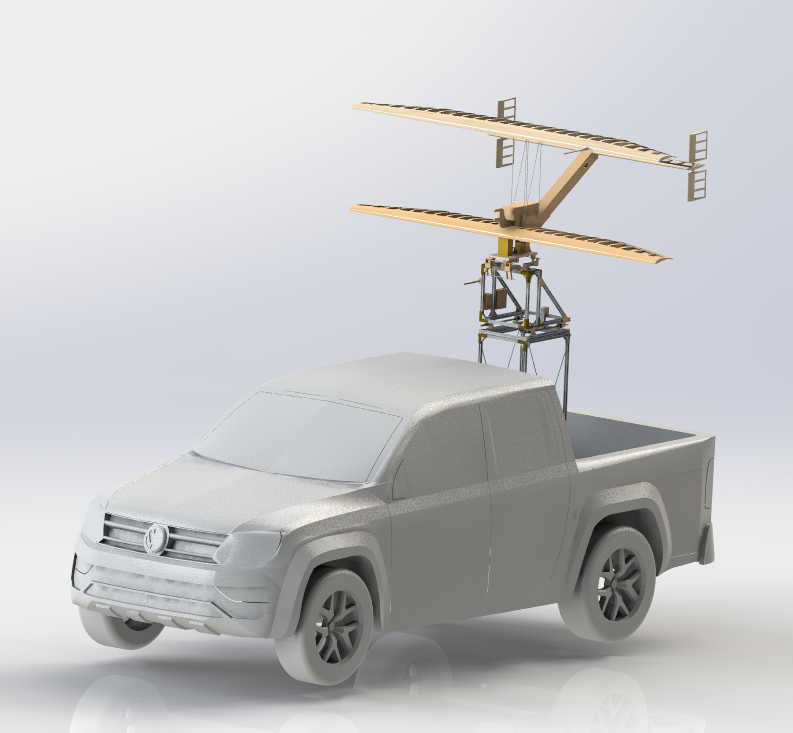
\includegraphics[width=.8\linewidth]{figuras/renders/aviao_no_carro.png}
    \caption{Renderização da bancada experimental desenvolvida neste trabalho com um VANT instalado como componente a ser carcterizado. Fonte: O autor..}
    \label{fig:render_bancada_aviao_carro}
\end{figure}

A proposta deste trabalho consiste no projeto e análise de uma bancada para medição de esforços aerodinâmicos sem túnel de vento, a ser utilizada para a caracterização aerodinâmica de componentes de VANTs. Tal bancada consiste de células de carga, tubos de pitot e outros sensores, e é embarcada em um veiculo automotor, que ao ser movimentado faz com que um escoamento surja sobre o componente a ser experimentado.

\section{Objetivo geral}

Desenvolvimento de uma bancada de baixo custo para caracterização aerodinâmica de componentes de VANTs, visando a eliminação ou minimização da necessidade de um túnel de vento, reduzindo o ciclo de otimização de projeto.
